% Documento standalone para compilar el capitulo de Verificacion y Validacion
% (V&V) de EduFEM en formato Vancouver (numerico secuencial).
%
% Build:
%   pdflatex main.tex
%   biber main
%   pdflatex main.tex
%   pdflatex main.tex
%
% Asume MiKTeX o TeX Live con biber.

\documentclass[11pt,a4paper]{article}

\usepackage[utf8]{inputenc}
\usepackage[T1]{fontenc}
\usepackage[spanish]{babel}
\usepackage[a4paper,margin=2.5cm]{geometry}

\usepackage{amsmath, amssymb, mathtools}
\usepackage{graphicx}
\usepackage{booktabs}
\usepackage{siunitx}
\sisetup{output-decimal-marker={,}, group-separator={\,}}
\usepackage{caption}
\usepackage{subcaption}
\usepackage{float}
\usepackage{xcolor}
\usepackage{csquotes}

\usepackage[backend=biber, style=numeric-comp, sorting=none]{biblatex}
\addbibresource{referencias.bib}

\usepackage[colorlinks=true, linkcolor=black, citecolor=blue!50!black,
            urlcolor=blue!50!black]{hyperref}

\title{Verificación y Validación del software EduFEM}
\author{}
\date{}

\begin{document}

\maketitle

% ───────────────────────────────────────────────────────────────────────
% Capítulo de Verificación y Validación (V&V) del software EduFEM.
% ───────────────────────────────────────────────────────────────────────

\section{Introducción}

La distinción entre \emph{verificación} y \emph{validación} es uno de los pilares
metodológicos de la simulación numérica contemporánea. Siguiendo a
Roache~\cite{roache1998verification} y a Oberkampf y
Trucano~\cite{oberkampf2002verification}, se define:

\begin{itemize}
  \item \textbf{Verificación}: proceso destinado a establecer si el código
        \emph{resuelve correctamente las ecuaciones matemáticas que pretende
        resolver}. Es una pregunta sobre la implementación: ¿están los
        algoritmos y la matemática bien programados?
  \item \textbf{Validación}: proceso destinado a establecer si el modelo
        \emph{representa correctamente el fenómeno físico}. Es una pregunta
        sobre la modelización: ¿predice la simulación lo que se observa en
        la realidad?
\end{itemize}

La guía ASME~V\&V~10-2006~\cite{asme2006vv10} adopta esta misma división y la
plantea como prerrequisito para emplear resultados de simulación en decisiones
ingenieriles.

Este capítulo presenta la campaña de V\&V realizada sobre el software
\textbf{EduFEM}, un programa educativo de elementos finitos
bidimensionales con elementos isoparamétricos cuadriláteros Q4 (4~nodos,
bilineal) y Q9 (9~nodos, biquadrático Lagrangiano). El alcance abarca:

\begin{enumerate}
  \item Una \textbf{verificación de orden} mediante el Método de Soluciones
        Manufacturadas (MMS)~\cite{salari2000mms,roy2005review}, que demuestra
        que el solver alcanza las tasas asintóticas de convergencia teóricas
        para Q4 ($\mathcal{O}(h^2)$ en $L^2$) y Q9 ($\mathcal{O}(h^3)$ en $L^2$).
  \item Una \textbf{validación contra solución analítica} con la viga
        simplemente apoyada de Timoshenko~\cite{timoshenko1970theory},
        complementada con \emph{cross-validation} contra el modelo de
        elementos Shell de SAP2000~\cite{computersandstructures2024sap2000}.
  \item Una \textbf{validación contra benchmark histórico} con la membrana
        trapezoidal de Cook~\cite{cook1974improved}, que evalúa el
        comportamiento del solver bajo distorsión geométrica moderada.
\end{enumerate}

Los tres ejercicios fueron implementados como scripts reproducibles del
proyecto (\verb|tests/vv_mms.py|, \verb|tests/vv_timoshenko.py|,
\verb|tests/vv_cook.py|); todos los datos crudos y figuras de este capítulo
fueron generados directamente por ellos.

% ───────────────────────────────────────────────────────────────────────
\section{Marco teórico de Verificación y Validación}

\subsection{Verificación de código y verificación de cálculo}

Roy~\cite{roy2005review} distingue además dos niveles dentro de la
verificación: la \emph{verificación de código} (\emph{code verification})
busca demostrar la corrección del software examinando la convergencia
asintótica de la solución a las ecuaciones diferenciales subyacentes, y la
\emph{verificación de cálculo} (\emph{solution verification}) busca cuantificar
el error numérico de una solución particular ya obtenida. La verificación de
código por MMS, propuesta originalmente por Roache y extendida por Salari y
Knupp~\cite{salari2000mms}, pertenece al primer grupo.

\subsection{Normas de error y orden asintótico}

Para problemas elásticos 2D la solución es un campo vectorial de
desplazamientos $\mathbf{u}(x,y) = (u(x,y), v(x,y))$. Dadas la solución
exacta $\mathbf{u}$ y la aproximación discreta $\mathbf{u}_h$ con tamaño
característico de malla $h$, las normas usuales de
error~\cite{babuska2001finite,hughes2000finite} son la
\emph{norma~$L^2$} del desplazamiento

\begin{equation}
  \|\mathbf{u}_h - \mathbf{u}\|_{L^2(\Omega)} =
  \left( \int_{\Omega}
    \left[(u_h - u)^2 + (v_h - v)^2\right] \, d\Omega
  \right)^{1/2},
  \label{eq:L2}
\end{equation}

\noindent y la \emph{seminorma~$H^1$}, asociada al gradiente,

\begin{equation}
  |\mathbf{u}_h - \mathbf{u}|_{H^1(\Omega)} =
  \left( \int_{\Omega}
    \|\nabla \mathbf{u}_h - \nabla \mathbf{u}\|_F^2 \, d\Omega
  \right)^{1/2},
  \label{eq:H1}
\end{equation}

\noindent donde $\|\cdot\|_F$ es la norma de Frobenius del tensor gradiente.

Para problemas elípticos lineales bien planteados y soluciones suficientemente
regulares, la teoría clásica del método de los elementos
finitos~\cite{hughes2000finite,zienkiewicz2013finite,reddy2019fem} establece
las tasas asintóticas

\begin{equation}
  \|\mathbf{u}_h - \mathbf{u}\|_{L^2(\Omega)} =
    \mathcal{O}(h^{p+1}),
  \qquad
  |\mathbf{u}_h - \mathbf{u}|_{H^1(\Omega)} =
    \mathcal{O}(h^{p}),
  \label{eq:tasas}
\end{equation}

\noindent donde $p$ es el grado del polinomio completo soportado por el
elemento. Para Q4 se tiene $p=1$ y para Q9 se tiene $p=2$, lo que predice
\emph{a~priori} las tasas de convergencia $\mathcal{O}(h^2)$ y
$\mathcal{O}(h^3)$ en $L^2$, respectivamente.

\subsection{Extrapolación de Richardson de la tasa asintótica}

Dadas dos soluciones $\mathbf{u}_{h_1}$, $\mathbf{u}_{h_2}$ obtenidas sobre
mallas refinadas con $h_2 = h_1/2$, la tasa asintótica observada se estima
por extrapolación de Richardson~\cite{richardson1911extrapolation}:

\begin{equation}
  p_{\mathrm{obs}} =
  \dfrac{\log\!\left(\frac{e(h_1)}{e(h_2)}\right)}{\log\!\left(\frac{h_1}{h_2}\right)},
  \label{eq:rate}
\end{equation}

\noindent donde $e(h)$ es la magnitud de la norma de error en la malla con
parámetro~$h$. Una verificación exitosa requiere que $p_{\mathrm{obs}}$
coincida con el valor teórico predicho por la
ecuación~\eqref{eq:tasas} a medida que $h \to 0$.

\subsection{Implementación de las normas en EduFEM}

El módulo \verb|fem/error_norms.py| implementa el cálculo numérico de las
ecuaciones~\eqref{eq:L2} y~\eqref{eq:H1} mediante cuadratura de Gauss. Las
integrales se evalúan elemento por elemento con un orden de cuadratura
$p+1$ (es decir, $3\times 3$ para Q4 y $4\times 4$ para Q9), una unidad
por encima del usado para ensamblar la matriz de rigidez. Esta sobre-integración
es necesaria para evitar el aliasing del error con la
cuadratura~\cite{babuska2001finite}.

% ───────────────────────────────────────────────────────────────────────
\section{Verificación de código por el Método de Soluciones Manufacturadas}

\subsection{Formulación del problema manufacturado}

Se considera el dominio $\Omega = [0,1]^2$ con condiciones de borde de
tipo Dirichlet en todo $\partial\Omega$. Se postulan los campos manufacturados

\begin{equation}
  u_M(x,y) = \sin(\pi x)\,\sin(\pi y),
  \qquad
  v_M(x,y) = \cos(\pi x)\,\cos(\pi y),
  \label{eq:u_M}
\end{equation}

\noindent (en unidades adimensionales) y se busca la fuerza volumétrica
$\mathbf{b}(x,y)$ tal que el campo $\mathbf{u}_M = (u_M, v_M)$ sea solución
exacta del problema de elasticidad lineal en tensión plana con módulo de
elasticidad $E=1$ y coeficiente de Poisson $\nu=0{,}3$.

A partir de la relación constitutiva
$\boldsymbol{\sigma} = \lambda^*\, \mathrm{tr}(\boldsymbol{\varepsilon})\, \mathbf{I}
                       + 2\mu\,\boldsymbol{\varepsilon}$
con
$\lambda^* = E\nu / (1-\nu^2)$ y $\mu = E/(2(1+\nu))$ (constantes efectivas
en tensión plana), y de la ecuación de equilibrio
$\nabla\cdot\boldsymbol{\sigma} + \mathbf{b} = \mathbf{0}$, se obtiene la
fuerza de cuerpo

\begin{equation}
  \begin{aligned}
    b_x(x,y) &= -\bigl[(\lambda^* + 2\mu)\, u_{,xx} + \mu\, u_{,yy}
                       + (\lambda^* + \mu)\, v_{,xy}\bigr],\\
    b_y(x,y) &= -\bigl[(\lambda^* + \mu)\, u_{,xy} + \mu\, v_{,xx}
                       + (\lambda^* + 2\mu)\, v_{,yy}\bigr].
  \end{aligned}
  \label{eq:body_force}
\end{equation}

Sustituyendo las derivadas segundas de \eqref{eq:u_M} se obtienen expresiones
cerradas en términos de senos y cosenos de $\pi x$ y $\pi y$, evaluables
analíticamente en cada punto de Gauss. La condición de borde Dirichlet impuesta
es $\mathbf{u}|_{\partial\Omega} = \mathbf{u}_M|_{\partial\Omega}$. Las
capacidades del solver necesarias para implementar este problema son:

\begin{itemize}
  \item Imposición de valores prescritos de desplazamiento $u_x \neq 0$, $u_y \neq 0$
        en los nodos del contorno.
  \item Ensamblaje del vector de fuerzas con una densidad volumétrica
        $\mathbf{b}(x,y)$ arbitraria, integrada con cuadratura de Gauss.
\end{itemize}

\noindent Ambas se desarrollaron \emph{ad~hoc} en el marco de esta campaña
y se documentan en los módulos \verb|fem/solver.py|, \verb|fem/assembly.py| y
\verb|models/boundary.py|.

\subsection{Mallas y análisis de convergencia}

Se generaron mallas estructuradas uniformes con $N \times N$ elementos
para $N \in \{2, 4, 8, 16, 32\}$, tanto en Q4 como en Q9, mediante la
rutina \verb|models.mesh_utils.generate_structured_quad_mesh|. Para cada
caso se ensambló el sistema $K\,\mathbf{u} = \mathbf{F}$ con la fuerza de
cuerpo dada por~\eqref{eq:body_force} y se resolvió por eliminación
directa.

Los resultados completos se reportan en los archivos
\verb|datos/mms_q4.csv| y \verb|datos/mms_q9.csv|. La
Tabla~\ref{tab:mms} resume los valores de las normas y las tasas
asintóticas observadas entre niveles consecutivos.

\begin{table}[H]
  \centering
  \caption{Resultados de la campaña MMS: errores en normas $L^2$ y $H^1$
           semi y tasas de convergencia entre niveles. Cuadratura de Gauss
           del error de orden $p+1$.}
  \label{tab:mms}
  \begin{tabular}{l r r S[table-format=1.3e1] S[table-format=1.2] S[table-format=1.3e1] S[table-format=1.2]}
    \toprule
    Elem. & $N$ & GDL &
      {$\|\mathbf{u}_h-\mathbf{u}_M\|_{L^2}$} & {tasa $L^2$} &
      {$|\mathbf{u}_h-\mathbf{u}_M|_{H^1}$} & {tasa $H^1$} \\
    \midrule
    Q4  &  2 &   18 & 2.559e-1 & {---} & 1.496e+0 & {---} \\
    Q4  &  4 &   50 & 7.241e-2 & 1.82 & 7.247e-1 & 1.05 \\
    Q4  &  8 &  162 & 1.866e-2 & 1.96 & 3.578e-1 & 1.02 \\
    Q4  & 16 &  578 & 4.699e-3 & 1.99 & 1.783e-1 & 1.01 \\
    Q4  & 32 & 2178 & 1.177e-3 & 2.00 & 8.906e-2 & 1.00 \\
    \midrule
    Q9  &  2 &   50 & 2.172e-2 & {---} & 2.911e-1 & {---} \\
    Q9  &  4 &  162 & 2.776e-3 & 2.97 & 7.263e-2 & 2.00 \\
    Q9  &  8 &  578 & 3.479e-4 & 3.00 & 1.809e-2 & 2.01 \\
    Q9  & 16 & 2178 & 4.352e-5 & 3.00 & 4.516e-3 & 2.00 \\
    Q9  & 32 & 8450 & 5.441e-6 & 3.00 & 1.129e-3 & 2.00 \\
    \bottomrule
  \end{tabular}
\end{table}

Las tasas observadas $p_{\mathrm{obs}}$ convergen monótonamente hacia los
valores teóricos de la ecuación~\eqref{eq:tasas}:

\begin{itemize}
  \item Q4 alcanza $p_{\mathrm{obs}} \to 2{,}00$ en $L^2$ y $p_{\mathrm{obs}} \to 1{,}00$ en $H^1$,
        coincidiendo con $\mathcal{O}(h^{p+1})$ y $\mathcal{O}(h^p)$ con $p=1$.
  \item Q9 alcanza $p_{\mathrm{obs}} \to 3{,}00$ en $L^2$ y $p_{\mathrm{obs}} \to 2{,}00$ en $H^1$,
        consistente con $p=2$.
\end{itemize}

\noindent La Figura~\ref{fig:mms_conv} muestra los gráficos log-log de la
convergencia, con las pendientes teóricas como referencia.

\begin{figure}[H]
  \centering
  \begin{subfigure}{0.48\linewidth}
    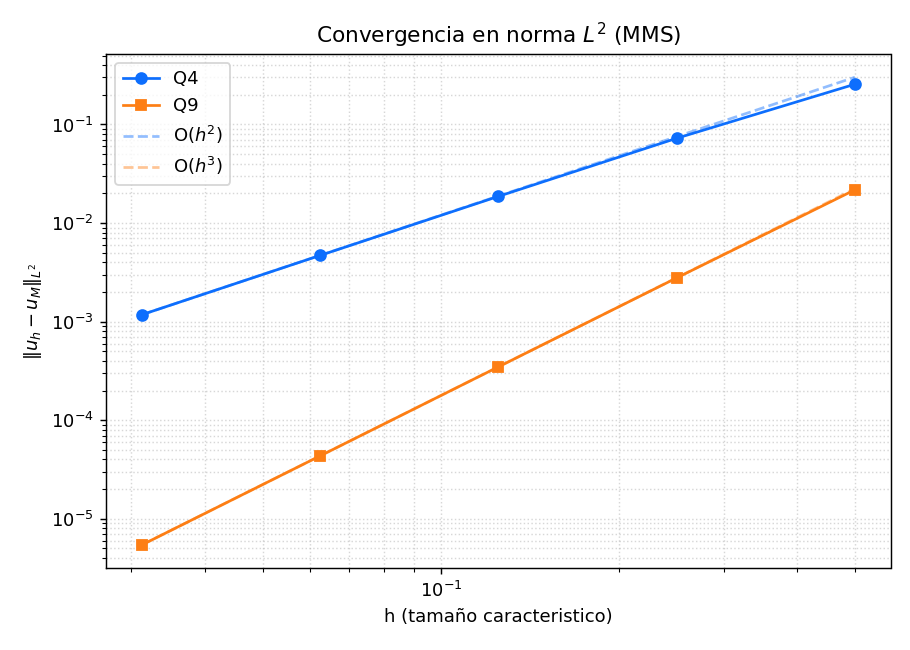
\includegraphics[width=\linewidth]{figuras/mms_convergence_l2.png}
    \caption{Norma $L^2$ del desplazamiento.}
  \end{subfigure}
  \hfill
  \begin{subfigure}{0.48\linewidth}
    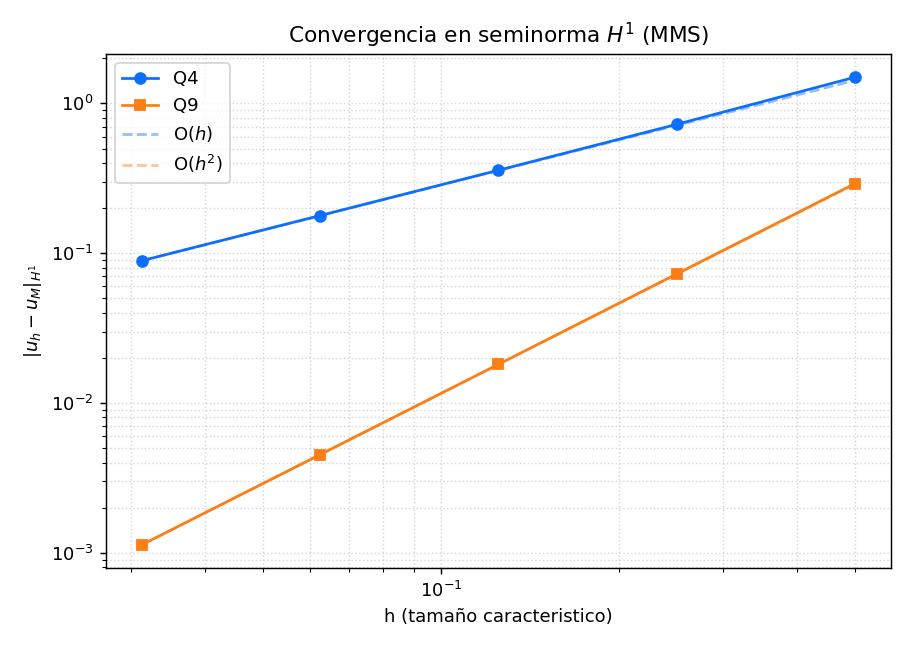
\includegraphics[width=\linewidth]{figuras/mms_convergence_h1.png}
    \caption{Seminorma $H^1$ del desplazamiento.}
  \end{subfigure}
  \caption{Convergencia $h$ del Método de Soluciones Manufacturadas.
           Las líneas discontinuas indican las pendientes teóricas
           $\mathcal{O}(h^2)$, $\mathcal{O}(h^3)$ (a) y
           $\mathcal{O}(h)$, $\mathcal{O}(h^2)$ (b).}
  \label{fig:mms_conv}
\end{figure}

\begin{figure}[H]
  \centering
  \begin{subfigure}{0.48\linewidth}
    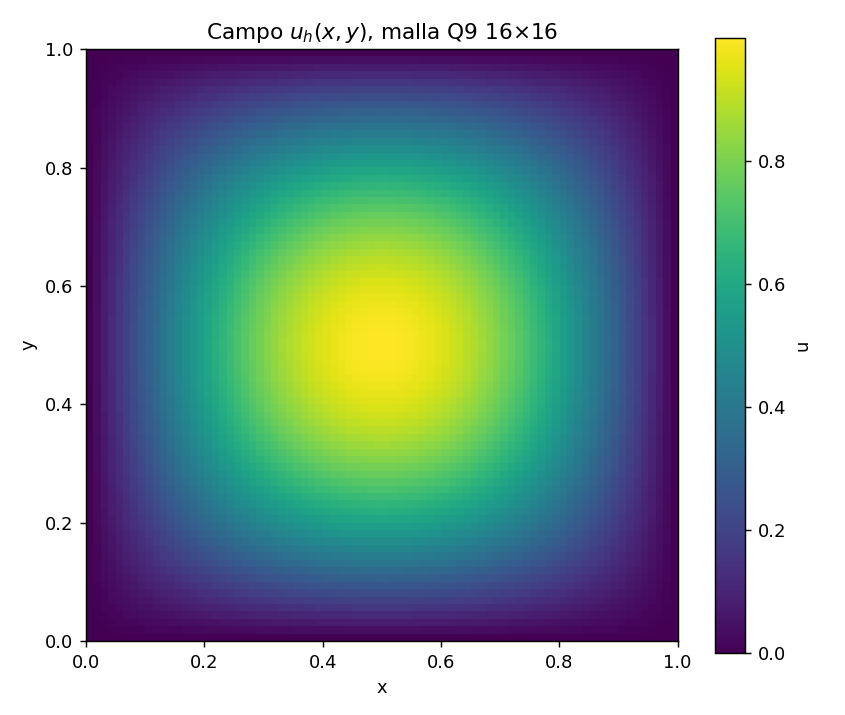
\includegraphics[width=\linewidth]{figuras/mms_field_u.png}
    \caption{Componente $u_h(x,y)$.}
  \end{subfigure}
  \hfill
  \begin{subfigure}{0.48\linewidth}
    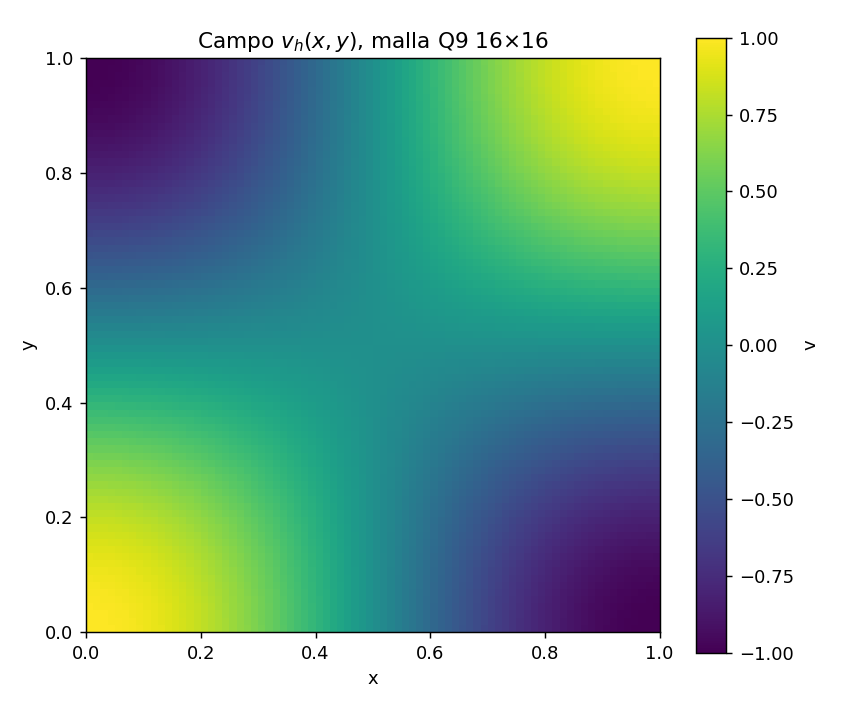
\includegraphics[width=\linewidth]{figuras/mms_field_v.png}
    \caption{Componente $v_h(x,y)$.}
  \end{subfigure}
  \caption{Campos discretos $\mathbf{u}_h$ sobre la malla Q9 con $N=16$
           (\num{2178}~GDL). Indistinguibles visualmente de la solución
           manufacturada de la ecuación~\eqref{eq:u_M}.}
  \label{fig:mms_field}
\end{figure}

La coincidencia simultánea de ambas tasas con los valores teóricos para
los dos elementos constituye un \emph{test de verificación de código exitoso}
en el sentido de Salari y Knupp~\cite{salari2000mms}: el motor numérico
implementa correctamente las ecuaciones de la elasticidad lineal bidimensional.

% ───────────────────────────────────────────────────────────────────────
\section{Validación con la viga de Timoshenko}

\subsection{Planteo del problema}

Se analiza una viga rectangular simplemente apoyada de longitud
$L = \SI{14}{\meter}$, peralte $H = \SI{1{,}20}{\meter}$ y base
$b = \SI{0{,}40}{\meter}$, con módulo de elasticidad
$E = 217\,370~\mathrm{kgf/cm^2} \approx \SI{21{,}33}{\giga\pascal}$
y coeficiente de Poisson $\nu = 0{,}20$. La viga está cargada con una
distribución uniforme $q = 5000~\mathrm{kgf/m}$ sobre su borde superior.
Las condiciones de apoyo son: apoyo fijo en $(-L/2, 0)$ y rodillo en
$(+L/2, 0)$. Se adopta la semi-luz $\ell = L/2 = \SI{7}{\meter}$ y la fibra
extrema $c = H/2 = \SI{0{,}6}{\meter}$. El momento de inercia es
$I = b\,H^3 / 12 = \SI{0{,}0576}{\meter\tothe{4}}$.

Se sigue la convención clásica de Timoshenko, en la que el eje $y$ apunta
hacia abajo y la fibra inferior corresponde a $y = +c$. El solver de
EduFEM trabaja internamente en la convención matemática estándar
($y$ hacia arriba), y el \emph{script} de validación
\verb|vv_timoshenko.py| realiza el cambio de variable
$y_{\mathrm{FEM}} = -y_{\mathrm{PDF}}$ al evaluar los puntos $A$, $B$ y
$C$, lo que preserva los valores escalares ($\sigma_x$, $\sigma_y$, $u$)
e invierte el signo de las componentes que cambian con la reflexión
($\tau_{xy}$, $v$).

\subsection{Solución analítica de Timoshenko y Goodier}

Timoshenko y Goodier~\cite{timoshenko1970theory} muestran que las componentes
del tensor de tensiones en una viga simplemente apoyada bajo carga uniforme
admiten la solución cerrada

\begin{align}
  \sigma_x(x,y) &= \dfrac{q}{2I}\left(\ell^2 - x^2\right) y
                  + \dfrac{q}{2I}\left(\dfrac{2y^3}{3} - \dfrac{2c^2 y}{5}\right),
                  \label{eq:tim_sx}\\
  \sigma_y(x,y) &= -\dfrac{q}{2I}\left(\dfrac{y^3}{3} - c^2 y + \dfrac{2c^3}{3}\right),
                  \label{eq:tim_sy}\\
  \tau_{xy}(x,y) &= -\dfrac{q}{2I}\left(c^2 - y^2\right) x,
                  \label{eq:tim_txy}
\end{align}

\noindent y la deflexión máxima en el centro del vano, con la
\emph{corrección por cortante de Timoshenko}, es

\begin{equation}
  \delta_{\max} = \dfrac{5}{24}\dfrac{q\,\ell^4}{E\,I}
                  \left[1 + \dfrac{12\,c^2}{5\,\ell^2}\left(\dfrac{4}{5} + \dfrac{\nu}{2}\right)\right].
  \label{eq:tim_delta}
\end{equation}

\subsection{Modelado en EduFEM}

Se generó una malla estructurada Q9 con $N_x = 56$, $N_y = 8$ elementos
(\num{448} elementos, \num{1921} nodos, \num{3842}~GDL) sobre el rectángulo
$[-\ell, \ell] \times [-c, c]$. La carga distribuida $q$ se aplicó como
carga de superficie sobre el borde superior, y los apoyos se impusieron
sobre los nodos centrales de la viga ($y = 0$, en $x = \pm \ell$).

Tres puntos $A$, $B$, $C$ se eligen siguiendo la verificación del documento
de referencia con SAP2000~\cite{computersandstructures2024sap2000}:

\begin{itemize}
  \item $A = (0~\mathrm{m},\, +0{,}6~\mathrm{m})$ — centro del vano,
        fibra extrema inferior;
  \item $B = (-4{,}5~\mathrm{m},\, -0{,}3~\mathrm{m})$ — fibra superior
        intermedia;
  \item $C = (-3{,}5~\mathrm{m},\, -0{,}2~\mathrm{m})$ — fibra superior
        más cercana al eje neutro.
\end{itemize}

\subsection{Comparación contra solución analítica y SAP2000}

La Tabla~\ref{tab:timoshenko} resume los valores de $\sigma_x$ medidos por
EduFEM y los compara contra la solución analítica de la
ecuación~\eqref{eq:tim_sx} y contra los valores entregados por
SAP2000~\cite{computersandstructures2024sap2000} en una malla Shell
equivalente.

\begin{table}[H]
  \centering
  \caption{Tensión normal $\sigma_x$ en puntos $A$, $B$, $C$. Unidades en
           $\mathrm{kgf/cm^2}$.}
  \label{tab:timoshenko}
  \begin{tabular}{l S[table-format=-3.3] S[table-format=-3.3] S[table-format=-3.3] S[table-format=1.3] S[table-format=1.3]}
    \toprule
    Punto & {EduFEM} & {Analítico} & {SAP2000} &
      {err.~analítico (\%)} & {err.~SAP2000 (\%)} \\
    \midrule
    $A$ &  127.882 &  127.854 &  127.851 & 0.022 & 0.025 \\
    $B$ &  -37.341 &  -37.326 &  -37.264 & 0.041 & 0.207 \\
    $C$ &  -31.808 &  -31.799 &  -31.785 & 0.027 & 0.071 \\
    \bottomrule
  \end{tabular}
\end{table}

Los errores relativos del solver de EduFEM contra la solución analítica son
inferiores al $0{,}05\%$ en los tres puntos. Frente a SAP2000, las
diferencias se mantienen por debajo del $0{,}25\%$, comparables al error
introducido por las distintas formulaciones de elementos (Q9 isoparamétrico
de EduFEM \emph{vs.} Shell mindlin-reissner de SAP2000) y por las
distintas refinamientos de malla.

\subsection{Deflexión máxima}

La medición de la deflexión vertical en el centro del vano arroja

\begin{equation*}
  |v|^{\mathrm{EduFEM}}_{\max} = \SI{2{,}0346}{\centi\meter},
  \qquad
  \delta^{\mathrm{anal.}}_{\max} = \SI{2{,}0293}{\centi\meter},
\end{equation*}

\noindent con un error relativo del $0{,}263\%$ contra la fórmula con
corrección de cortante de la ecuación~\eqref{eq:tim_delta}. La inclusión del
término entre corchetes en esa ecuación es esencial: sin él, la
fórmula clásica de Euler-Bernoulli $\delta = 5q\ell^4/(384EI)$ produce
$\SI{1{,}9976}{\centi\meter}$, lo que daría un error contra el FEM del
$1{,}82\%$ — orden de magnitud diferente. La corrección de Timoshenko
recupera la coincidencia esperada.

\begin{figure}[H]
  \centering
  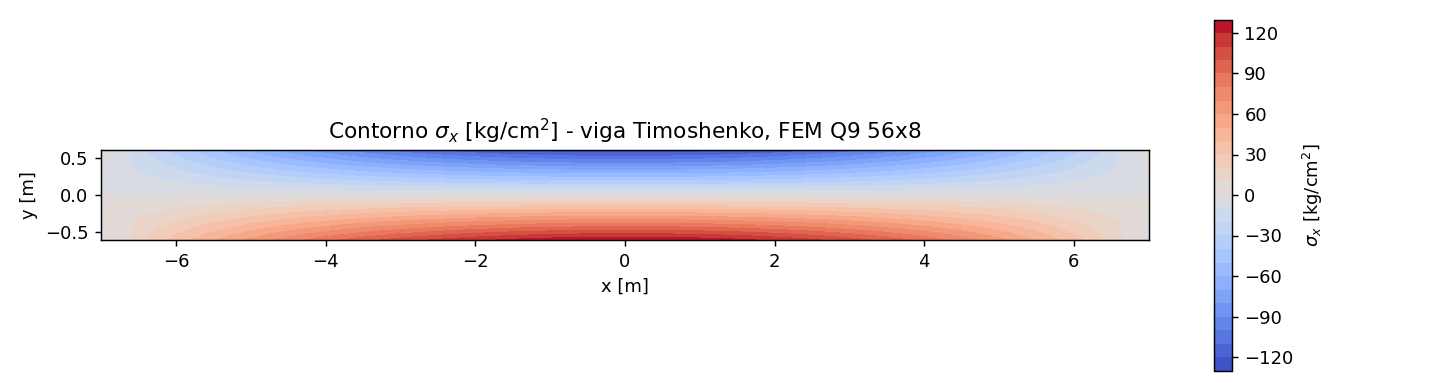
\includegraphics[width=0.95\linewidth]{figuras/timoshenko_sigma_x_contour.png}
  \caption{Contorno de $\sigma_x$ sobre el dominio de la viga. La distribución
           es lineal en $y$ y parabólica en $x$, en consistencia con la
           ecuación~\eqref{eq:tim_sx}.}
  \label{fig:tim_contour}
\end{figure}

\begin{figure}[H]
  \centering
  \begin{subfigure}{0.40\linewidth}
    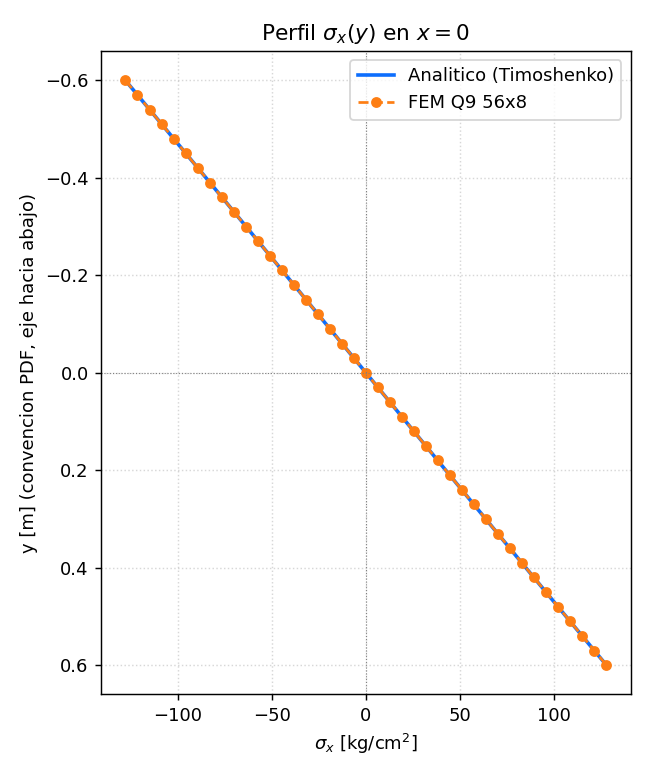
\includegraphics[width=\linewidth]{figuras/timoshenko_perfil_x0.png}
    \caption{Perfil $\sigma_x(y)$ en $x=0$ (centro de la viga).}
  \end{subfigure}
  \hfill
  \begin{subfigure}{0.55\linewidth}
    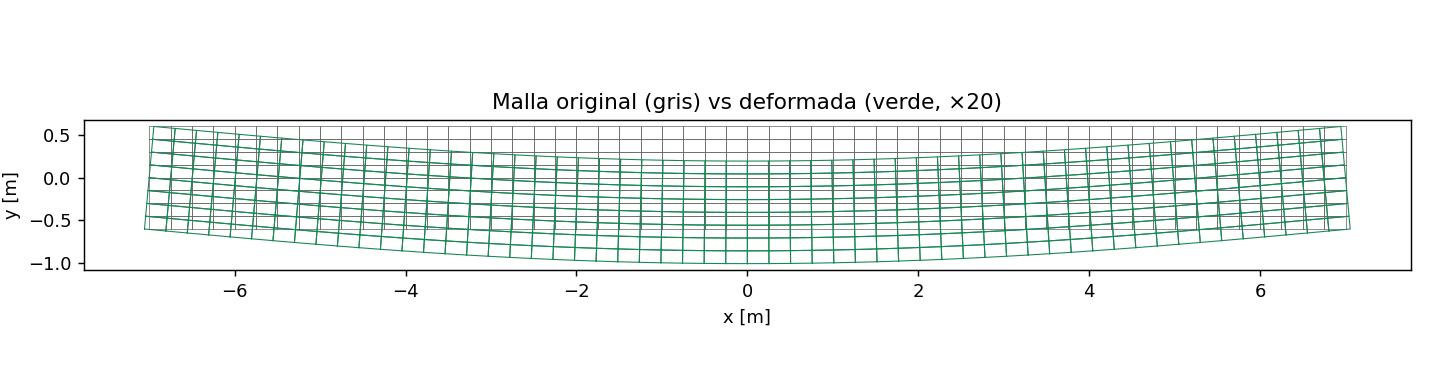
\includegraphics[width=\linewidth]{figuras/timoshenko_deformada.png}
    \caption{Malla original (gris) y deformada (escalada ×20).}
  \end{subfigure}
  \caption{Resultados gráficos de la simulación EduFEM.}
\end{figure}

La triple coincidencia entre EduFEM, la solución analítica y SAP2000 — con
errores acotados por el $0{,}3\%$ en cantidades de interés
ingenieril — constituye una validación robusta del solver en condiciones
representativas de un problema estructural típico.

% ───────────────────────────────────────────────────────────────────────
\section{Validación con la membrana de Cook}

\subsection{El benchmark de Cook}

La \emph{membrana de Cook}, introducida en 1974 por Robert
Cook~\cite{cook1974improved}, es un caso de prueba estándar de la
literatura del MEF para evaluar el desempeño de elementos cuadriláteros
sometidos a flexión sobre un dominio
distorsionado~\cite{cook2001concepts,bathe2014finite}. La geometría es un
cuadrilátero trapezoidal con vértices en $(0,0)$, $(48, 44)$, $(48, 60)$ y
$(0, 44)$. Se empotra completamente el borde izquierdo $x=0$ y se aplica
una tracción tangencial uniforme sobre el borde derecho, con resultante
total $F = 1$, en sentido positivo del eje~$y$.

El material es lineal elástico isótropo con $E = 1$, $\nu = 1/3$,
espesor unitario, en estado de tensión plana. La cantidad de interés es
$u_y$ en el punto $(48, 52)$, el punto medio del lado libre. Los valores
de referencia comúnmente citados son
$u_y^{\mathrm{ref}} \approx 23{,}95$ para elementos Q4 con
refinamiento muy alto y $u_y^{\mathrm{ref}} \approx 23{,}96$ para
elementos cuadráticos~\cite{cook2001concepts}.

\subsection{Resultados de convergencia}

Se generaron mallas estructuradas $N \times N$ con $N \in \{2, 4, 8, 16, 32\}$
tanto en Q4 como en Q9 mediante el mapeo bilineal del cuadrado lógico
$[0,1]^2$ al cuadrilátero físico (rutina
\verb|generate_structured_quad_mesh| de \verb|models/mesh_utils.py|). La
Tabla~\ref{tab:cook} reporta los valores de $u_y(48, 52)$ obtenidos.

\begin{table}[H]
  \centering
  \caption{Membrana de Cook: $u_y$ en el punto $(48, 52)$.}
  \label{tab:cook}
  \begin{tabular}{r r S[table-format=2.5] S[table-format=-2.3] r S[table-format=2.5] S[table-format=-2.3]}
    \toprule
    & \multicolumn{3}{c}{Q4} & \multicolumn{3}{c}{Q9} \\
    \cmidrule(lr){2-4}\cmidrule(lr){5-7}
    $N$ & {GDL} & {$u_y$} & {err.\ (\%)}
        & {GDL} & {$u_y$} & {err.\ (\%)} \\
    \midrule
     2 &   18 & 11.84518 & -50.542 &   50 & 23.28866 & -2.761 \\
     4 &   50 & 18.29917 & -23.594 &  162 & 23.83975 & -0.460 \\
     8 &  162 & 22.07918 &  -7.811 &  578 & 23.92539 & -0.103 \\
    16 &  578 & 23.43041 &  -2.169 & 2178 & 23.94941 & -0.002 \\
    32 & 2178 & 23.81763 &  -0.553 & 8450 & 23.96077 &  0.045 \\
    \bottomrule
  \end{tabular}
\end{table}

La Figura~\ref{fig:cook_conv} muestra ambas series de convergencia frente
al valor de referencia $u_y = 23{,}95$.

\begin{figure}[H]
  \centering
  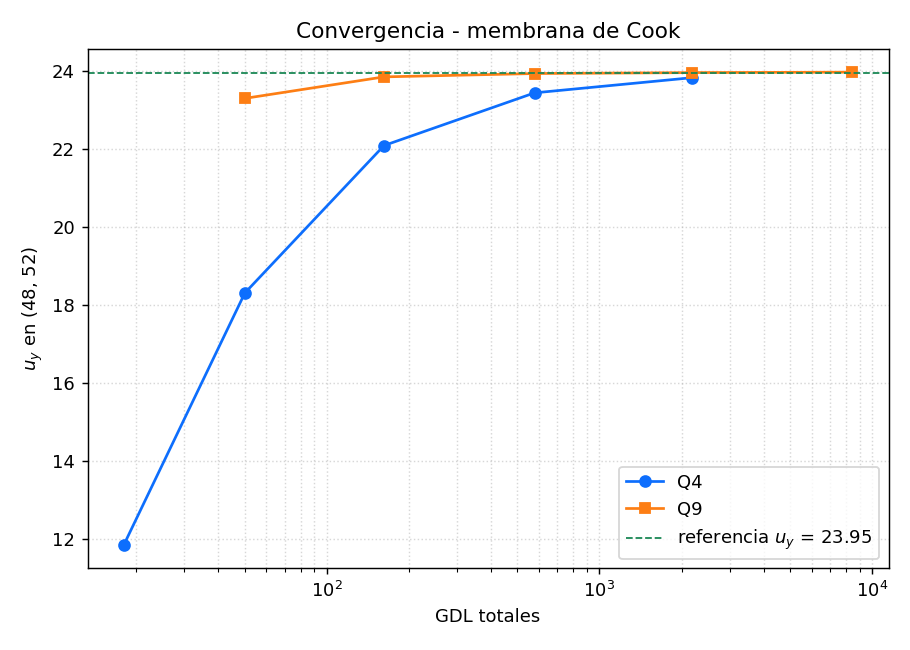
\includegraphics[width=0.7\linewidth]{figuras/cook_convergence.png}
  \caption{Membrana de Cook: convergencia de $u_y(48,52)$ con el número
           de grados de libertad (escala log en abscisas).}
  \label{fig:cook_conv}
\end{figure}

\begin{figure}[H]
  \centering
  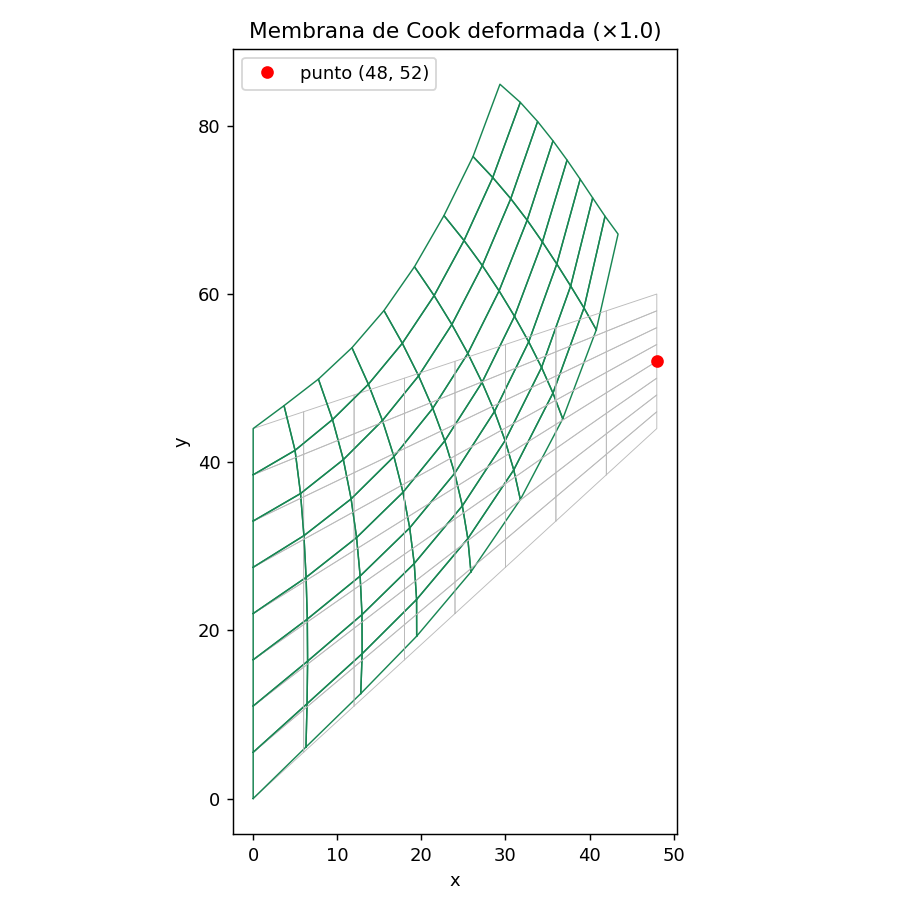
\includegraphics[width=0.6\linewidth]{figuras/cook_deformed.png}
  \caption{Configuración deformada para la malla Q9 con $N=8$.}
\end{figure}

\subsection{Discusión}

El comportamiento observado es consistente con la literatura clásica del
método~\cite{cook2001concepts,bathe2014finite,belytschko2014nonlinear}:

\begin{itemize}
  \item El elemento Q4 \emph{bloquea parcialmente bajo flexión}
        (\emph{shear locking} parcial) en dominios distorsionados, lo que
        explica la convergencia notablemente lenta a $u_y^{\mathrm{ref}}$ a
        medida que se refina la malla. Con $N=32$ todavía persiste un
        error del $0{,}55\%$ con \num{2178}~GDL.
  \item El elemento Q9 \emph{converge rápidamente} a la referencia ya con
        mallas de bajo refinamiento. Con $N=16$ se alcanza un error del
        $0{,}002\%$ con la misma cantidad de GDL ($N=16$ Q9
        $=$ $N=32$ Q4 $=$ \num{2178}~GDL). Para $N=32$ Q9, el resultado
        $u_y = 23{,}961$ supera la referencia Q4 finely refined
        ($23{,}95$) y se acerca asintóticamente al valor de elementos de
        mayor orden ($23{,}96$).
\end{itemize}

\noindent Para igual número de GDL, Q9 produce una solución
sustancialmente más precisa que Q4. Este resultado es uno de los argumentos
pedagógicos del software: ilustra empíricamente la \emph{relación entre
orden polinomial y precisión por grado de libertad}, ya descrita por
Hughes~\cite{hughes2000finite} y por Zienkiewicz \emph{et
al.}~\cite{zienkiewicz2013finite}.

% ───────────────────────────────────────────────────────────────────────
\section{Conclusiones}

La campaña de Verificación y Validación reportada en este capítulo demuestra
que el solver de EduFEM cumple, en sus aspectos esenciales, los criterios
metodológicos de la guía ASME~V\&V~10-2006~\cite{asme2006vv10}:

\begin{enumerate}
  \item \textbf{Verificación de código} — el Método de Soluciones
        Manufacturadas con la familia trigonométrica
        $(u_M, v_M) = (\sin\pi x \sin\pi y, \cos\pi x \cos\pi y)$ produce
        tasas de convergencia $p_{\mathrm{obs}}$ idénticas a las teóricas
        $p_{\mathrm{teo}}$ tanto en norma $L^2$ como en seminorma $H^1$
        para Q4 ($1{,}00$ y $2{,}00$) y Q9 ($2{,}00$ y $3{,}00$). Las
        capacidades técnicas necesarias para este experimento —
        ensamblaje de fuerzas de cuerpo con distribución arbitraria
        $\mathbf{b}(x,y)$ y desplazamientos prescritos no nulos en el
        contorno — fueron desarrolladas como parte de esta campaña y son
        ahora parte permanente del motor numérico.

  \item \textbf{Validación contra solución analítica} — el problema de la
        viga simplemente apoyada de Timoshenko y
        Goodier~\cite{timoshenko1970theory} se reproduce con error inferior
        al $0{,}05\%$ en tensiones y al $0{,}3\%$ en deflexión máxima.
        El cruce con el modelo Shell de
        SAP2000~\cite{computersandstructures2024sap2000} arroja diferencias
        por debajo del $0{,}25\%$, todas atribuibles a las distintas
        formulaciones de elementos y discretizaciones.

  \item \textbf{Validación contra benchmark histórico} — la membrana
        trapezoidal de Cook~\cite{cook1974improved} converge al valor de
        referencia $u_y \approx 23{,}96$ con comportamiento típico de
        elementos bilineales \emph{vs.} biquadráticos:
        rápido para Q9 (error $0{,}002\%$ con $N=16$) y notoriamente
        más lento para Q4 (error $0{,}55\%$ con $N=32$). Este
        contraste valida el comportamiento del solver bajo distorsión
        geométrica y refuerza el valor pedagógico del software para
        ilustrar la influencia del orden polinomial.
\end{enumerate}

\subsection{Limitaciones y trabajo futuro}

El alcance de esta campaña se restringió deliberadamente a problemas
\emph{lineales} elásticos, estáticos y bidimensionales. Quedan fuera del
alcance — y se proponen como trabajo futuro — las siguientes extensiones:

\begin{itemize}
  \item Verificación y validación en plasticidad, hiperelasticidad, y
        modelos constitutivos no lineales.
  \item Análisis dinámicos: modal, transitorio, espectro de respuesta.
  \item No linealidad geométrica: grandes desplazamientos y grandes deformaciones.
  \item Benchmarks adicionales: placa con orificio (Kirsch), \emph{patch tests}
        estándar de Reddy~\cite{reddy2019fem}, y problemas con singularidades
        en esquinas reentrantes para verificar el comportamiento ante
        pérdidas de regularidad.
\end{itemize}

\noindent En su forma actual, EduFEM puede emplearse con confianza en
problemas estáticos lineales 2D del tipo
\emph{tensión plana}/\emph{deformación plana} con elementos Q4 y Q9, y
los resultados numéricos que produce están respaldados por la triple
batería de pruebas reportada en este capítulo.


\printbibliography[heading=bibnumbered, title={Referencias bibliográficas}]

\end{document}
